
\documentclass[tikz,border=10pt]{standalone}
\usepackage[utf8]{inputenc}
\usepackage{fontawesome5} % Per le icone (Virus, Lucchetto, PC, DB)
\usepackage{xcolor}

% Librerie TikZ necessarie
\usetikzlibrary{positioning, arrows.meta, shapes.geometric, shadows.blur, backgrounds, fit, calc}

% Definizione colori personalizzati
\definecolor{GlassBlue}{RGB}{200, 230, 245}
\definecolor{MalwareRed}{RGB}{220, 50, 50}
\definecolor{LogGray}{RGB}{245, 245, 245}
\definecolor{CodeRed}{RGB}{180, 30, 30}

\begin{document}

\begin{tikzpicture}[
    node distance=2cm,
    font=\sffamily,
    >={Stealth[length=3mm]}, % Stile freccia
    % Stile per il testo dei log
    logtext/.style={
            align=left,
            font=\ttfamily\scriptsize,
            text width=6.5cm,
            anchor=north west
        }
    ]

    % ==============================
    % 1. DISEGNO IL CUBO (SANDBOX)
    % ==============================
    % Coordinate per proiezione pseudo-3D
    \coordinate (O) at (0,0);       % Origine fronte basso-sx
    \coordinate (W) at (3,0);       % Larghezza
    \coordinate (H) at (0,3);       % Altezza
    \coordinate (D) at (1.5,1.2);   % Profondità (vettore diagonale)

    % Calcolo i vertici del cubo
    \coordinate (A) at (O);
    \coordinate (B) at ($(O)+(W)$);
    \coordinate (C) at ($(O)+(W)+(H)$);
    \coordinate (D_front) at ($(O)+(H)$);

    \coordinate (A_back) at ($(O)+(D)$);
    \coordinate (B_back) at ($(O)+(W)+(D)$);
    \coordinate (C_back) at ($(O)+(W)+(H)+(D)$);
    \coordinate (D_back) at ($(O)+(H)+(D)$);

    % --- A. Facce Posteriori (Interne) ---
    \draw[fill=GlassBlue, opacity=0.3] (A_back) -- (B_back) -- (C_back) -- (D_back) -- cycle;
    \draw[gray!50] (A) -- (A_back);
    \draw[gray!50] (B) -- (B_back);

    % --- B. Contenuto (Malware e Icone) ---
    % Posiziono il virus al centro geometrico approssimativo
    \node[opacity=0.9] at ($(O) + 0.5*(W) + 0.4*(H) + 0.5*(D)$) {
        \scalebox{3}{\textcolor{MalwareRed}{\faVirus}}
    };

    % Lucchetto (un po' più in alto e indietro)
    \node[opacity=0.6] at ($(O) + 0.5*(W) + 0.8*(H) + 0.2*(D)$) {
        \scalebox{2}{\textcolor{darkgray}{\faLock}}
    };

    % Ingranaggi (piccoli a lato)
    \node[opacity=0.6] at ($(O) + 0.8*(W) + 0.6*(H) + 0.5*(D)$) {
        \scalebox{1.5}{\textcolor{gray}{\faCogs}}
    };

    % --- C. Facce Anteriori (Vetro) ---
    % Faccia Frontale
    \draw[thick, color=gray!80, fill=GlassBlue, fill opacity=0.2] (A) -- (B) -- (C) -- (D_front) -- cycle;
    % Faccia Superiore
    \draw[thick, color=gray!80, fill=GlassBlue, fill opacity=0.2] (D_front) -- (C) -- (C_back) -- (D_back) -- cycle;
    % Faccia Laterale Destra
    \draw[thick, color=gray!80, fill=GlassBlue, fill opacity=0.1] (B) -- (C) -- (C_back) -- (B_back) -- cycle;

    % Etichette Sandbox
    \node[above=0.5cm of C_back] (sb_title) {\textbf{Ambiente Sandbox}};
    \node[below=0.2cm of A] (sb_label) {Sandbox (Isolato)};


    % ==============================
    % 2. MONITORING SYSTEM
    % ==============================
    \node[right=2cm of B, align=center] (monitor) {
        \scalebox{3}{\textcolor{darkgray}{\faDesktop}} \\
        \vspace{0.2cm} \\
        \footnotesize Monitoring System
    };

    % Freccia dal cubo al monitor
    \draw[->, thick] ($(B)!0.5!(C)$) -- (monitor);


    % ==============================
    % 3. LOG LIST (Registrazione API)
    % ==============================
    % Creiamo un rettangolo con angoli arrotondati per simulare la finestra dei log
    \node[
        rectangle,
        rounded corners,
        draw=gray!50,
        fill=LogGray,
        thick,
        right=1.5cm of monitor,
        minimum width=7cm,
        minimum height=4cm,
        yshift=1cm,
        align=left
    ] (logbox) {};

    % Titolo sopra il box
    \node[above=0.1cm of logbox] {\textbf{Registrazione Chiamate API}};

    % Contenuto del Log (Uso un nodo interno per il testo formattato)
    \node[logtext] at ($(logbox.north west) + (0.3, -0.3)$) {
        10:01:32 -- \textbf{\textcolor{CodeRed}{CreateFile}} \\
        (C:\textbackslash Windows\textbackslash System32\textbackslash malicious.dll) \\[0.2cm]

        10:01:35 -- \textbf{\textcolor{CodeRed}{RegSetValueEx}} \\
        (HKCU\textbackslash Software\textbackslash Microsoft\textbackslash ...\textbackslash Run) \\[0.2cm]

        10:01:40 -- \textbf{\textcolor{CodeRed}{InternetOpenUrl}} \\
        (http://evil-server.com/data) \\[0.2cm]

        10:01:45 -- \textbf{\textcolor{CodeRed}{SocketConnect}} \\
        (192.168.1.100:4444)
    };

    % Freccia dal Monitor alla lista (leggermente curva)
    \draw[->, thick] (monitor.east) to[out=0, in=180] (logbox.west);


    % ==============================
    % 4. DATABASE (Output finale)
    % ==============================
    \node[below=1.5cm of logbox, align=center] (db) {
        \scalebox{3}{\textcolor{gray}{\faDatabase}} \\
        \vspace{0.1cm} \\
        \footnotesize Log Comportamentale
    };

    % Freccia dai log al DB
    \draw[->, thick] (logbox.south) -- (db.north);

\end{tikzpicture}
\end{document}